\chapter{Descrição do funcionamento do software}
% Os titulos dados aos capítulos são meros exemplos. Cada relatório deve adequar-se ao projeto desenvolvido.
\label{chap:desc-soft}
O jogo consiste numa nave que, controlada pelo jogador através do rato e do teclado, tem de destruir os asteróides existentes. Caso a nave não consiga destruir ou desviar-se dos asteróides, esta vai perdendo vida até ser destruída.
\linebreak
\linebreak
A nave movimenta-se num mapa esférico com limites bem definidos, caso a nave se movimente para fora dos limites do mapa, inicialmente aparecerá uma mensagem de aviso que se ignorada pelo jogador, este perderá o jogo tendo de começar de novo.
\linebreak
\linebreak
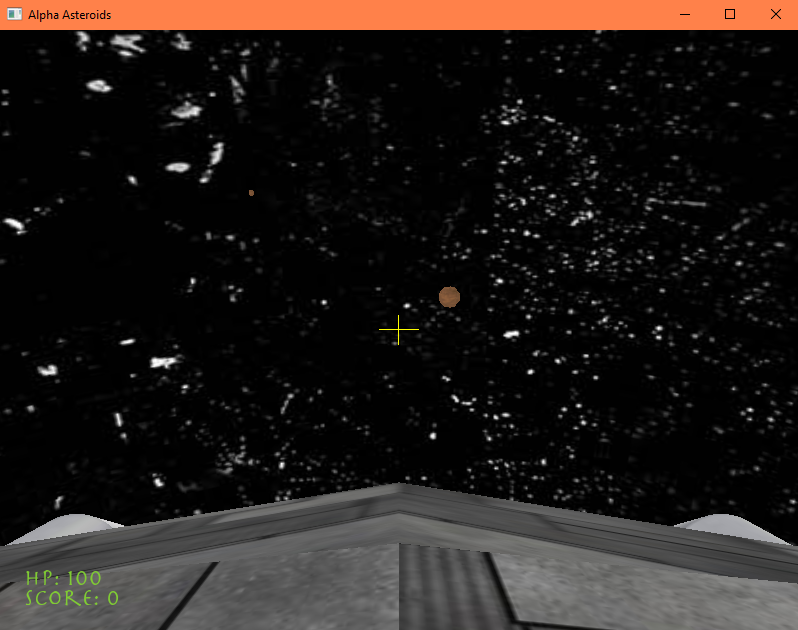
\includegraphics[scale=0.5]{jogo.png}